\chapter{Translation And The Genetic Code}\label{translation-and-the-genetic-code}

In molecular biology and genetics, \href{https://en.wikipedia.org/wiki/Translation_(biology)}{translation} is the process in which ribosomes in the cytoplasm or ER synthesize proteins after the process of transcription of DNA to RNA in the cell's nucleus. The entire process is called gene expression.

In translation, messenger RNA (mRNA) is decoded in the ribosome decoding center to produce a specific amino acid chain, or polypeptide. The polypeptide later folds into an active protein and performs its functions in the cell. The ribosome facilitates decoding by inducing the binding of complementary tRNA anticodon sequences to mRNA codons. The tRNAs carry specific amino acids that are chained together into a polypeptide a the mRNA passes through and is read by the ribosome.

Translation proceeds in three phases:

\begin{enumerate}
\def\labelenumi{\arabic{enumi}.}
\tightlist
\item
  \textbf{Initiation:} The ribosome assembles around the target mRNA. The first tRNA is attached at the start codon.
\item
  \textbf{Elongation:} The tRNA transfers an amino acid to the tRNA corresponding to the next codon. The ribosome then moves (translocates) to the next mRNA codon to continue the process, creating an amino acid chain.
\item
  \textbf{Termination:} When a peptidyl tRNA encounters a stop codon, then the ribosome folds the polypeptide into its final structure.
\end{enumerate}



\begin{figure}

{\centering 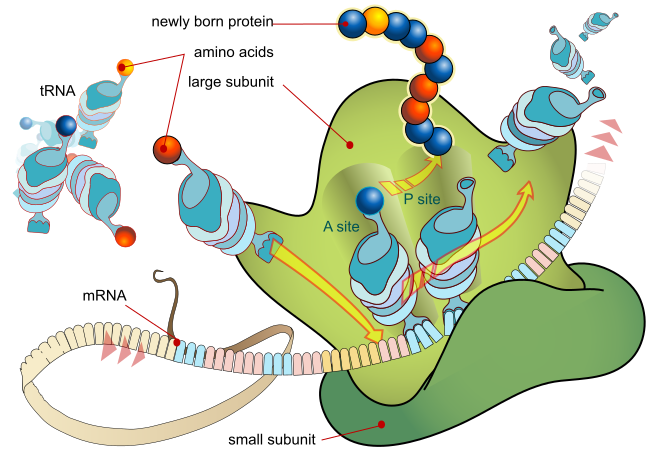
\includegraphics[width=0.7\linewidth]{./figures/translation/Ribosome_mRNA_translation_en} 

}

\caption{\href{https://commons.wikimedia.org/wiki/File:Ribosome_mRNA_translation_en.svg}{Diagram showing the translation of mRNA and the synthesis of proteins by a ribosome.}}\label{fig:translation}
\end{figure}

In prokaryotes, translation occurs in the cytosol, where the medium and small subunits of the ribosome bind to the tRNA. In eukaryotes, translation occurs in the cytosol or across the membrane of the endoplasmic reticulum in a process called co-translational translocation. In co-translational translocation, the entire ribosome/mRNA complex binds to the outer membrane of the rough endoplasmic reticulum (ER) and the new protein is synthesized and released into the ER; the newly created polypeptide can be stored inside the ER for future vesicle transport and secretion outside the cell, or immediately secreted.

Many types of transcribed RNA, such as transfer RNA, ribosomal RNA, and small nuclear RNA, do not undergo translation into proteins.

A number of antibiotics act by inhibiting translation. These include clindamycin, anisomycin, cycloheximide, chloramphenicol, tetracycline, streptomycin, erythromycin, and puromycin. Prokaryotic ribosomes have a different structure from that of eukaryotic ribosomes, and thus antibiotics can specifically target bacterial infections without any harm to a eukaryotic host's cells.

In 1954, Zamecnik and Hoagland discovered tRNA. In 1955, George E. Palade discovered ribosomes.

The basic process of translation is the addition of one amino acid at a time to the end of the polypeptide being formed. This process takes place inside the ribosome.

\hypertarget{eukaryotic-translation}{%
\section{Eukaryotic translation}\label{eukaryotic-translation}}

\hypertarget{initiation-3}{%
\subsection{Initiation}\label{initiation-3}}

Initiation of translation usually involves the interaction of certain key proteins, the initiation factors, with a special tag bound to the 5'-end of an mRNA molecule, the 5' cap, as well as with the 5' UTR. These proteins bind the small (40S) ribosomal subunit and hold the mRNA in place. eIF3 is associated with the 40S ribosomal subunit and plays a role in keeping the large (60S) ribosomal subunit from prematurely binding. eIF3 also interacts with the eIF4F complex, which consists of three other initiation factors: eIF4A, eIF4E, and eIF4G. eIF4G is a scaffolding protein that directly associates with both eIF3 and the other two components. eIF4E is the cap-binding protein. Binding of the cap by eIF4E is often considered the rate-limiting step of cap-dependent initiation, and the concentration of eIF4E is a regulatory nexus of translational control. Certain viruses cleave a portion of eIF4G that binds eIF4E, thus preventing cap-dependent translation to hijack the host machinery in favor of the viral (cap-independent) messages. eIF4A is an ATP-dependent RNA helicase that aids the ribosome by resolving certain secondary structures formed along the mRNA transcript. The poly(A)-binding protein (PABP) also associates with the eIF4F complex via eIF4G, and binds the poly-A tail of most eukaryotic mRNA molecules. This protein has been implicated in playing a role in circularization of the mRNA during translation. This 43S preinitiation complex (43S PIC) accompanied by the protein factors moves along the mRNA chain toward its 3'-end, in a process known as `scanning', to reach the start codon (typically AUG). In eukaryotes and archaea, the amino acid encoded by the start codon is methionine. The Met-charged initiator tRNA (Met-tRNAiMet) is brought to the P-site of the small ribosomal subunit by eukaryotic initiation factor 2 (eIF2). It hydrolyzes GTP, and signals for the dissociation of several factors from the small ribosomal subunit, eventually leading to the association of the large subunit (or the 60S subunit). The complete ribosome (80S) then commences translation elongation. Regulation of protein synthesis is partly influenced by phosphorylation of eIF2 (via the α subunit), which is a part of the eIF2-GTP-Met-tRNAiMet ternary complex (eIF2-TC). When large numbers of eIF2 are phosphorylated, protein synthesis is inhibited. This occurs under amino acid starvation or after viral infection. However, a small fraction of this initiation factor is naturally phosphorylated. Another regulator is 4EBP, which binds to the initiation factor eIF4E and inhibits its interactions with eIF4G, thus preventing cap-dependent initiation. To oppose the effects of 4EBP, growth factors phosphorylate 4EBP, reducing its affinity for eIF4E and permitting protein synthesis. While protein synthesis is globally regulated by modulating the expression of key initiation factors as well as the number of ribosomes, individual mRNAs can have different translation rates due to the presence of regulatory sequence elements. This has been shown to be important in a variety of settings including yeast meiosis and ethylene response in plants. In addition, recent work in yeast and humans suggest that evolutionary divergence in cis-regulatory sequences can impact translation regulation. Additionally, RNA helicases such as DHX29 and Ded1/DDX3 may participate in the process of translation initiation, especially for mRNAs with structured 5'UTRs.

Cap-independent initiation
The best-studied example of cap-independent translation initiation in eukaryotes is that by the Internal ribosome entry site (IRES). What differentiates cap-independent translation from cap-dependent translation is that cap-independent translation does not require the 5' cap to initiate scanning from the 5' end of the mRNA until the start codon. The ribosome can be trafficked to the start site by direct binding, initiation factors, and/or ITAFs (IRES trans-acting factors) bypassing the need to scan the entire 5' UTR. This method of translation has been found important in conditions that require the translation of specific mRNAs during cellular stress, when overall translation is reduced. Examples include factors responding to apoptosis and stress-induced responses.

\hypertarget{elongation-3}{%
\subsection{Elongation}\label{elongation-3}}

Elongation depends on eukaryotic elongation factors. At the end of the initiation step, the mRNA is positioned so that the next codon can be translated during the elongation stage of protein synthesis. The initiator tRNA occupies the P site in the ribosome, and the A site is ready to receive an aminoacyl-tRNA. During chain elongation, each additional amino acid is added to the nascent polypeptide chain in a three-step microcycle. The steps in this microcycle are (1) positioning the correct aminoacyl-tRNA in the A site of the ribosome, (2) forming the peptide bond and (3) shifting the mRNA by one codon relative to the ribosome. Unlike bacteria, in which translation initiation occurs as soon as the 5' end of an mRNA is synthesized, in eukaryotes such tight coupling between transcription and translation is not possible because transcription and translation are carried out in separate compartments of the cell (the nucleus and cytoplasm). Eukaryotic mRNA precursors must be processed in the nucleus (e.g., capping, polyadenylation, splicing) before they are exported to the cytoplasm for translation. Translation can also be affected by ribosomal pausing, which can trigger endonucleolytic attack of the mRNA, a process termed mRNA no-go decay. Ribosomal pausing also aids co-translational folding of the nascent polypeptide on the ribosome, and delays protein translation while it is encoding mRNA. This can trigger ribosomal frameshifting.

\hypertarget{termination-3}{%
\subsection{Termination}\label{termination-3}}

Termination of elongation depends on eukaryotic release factors. The process is similar to that of prokaryotic termination, but unlike prokaryotic termination, there is a universal release factor, eRF1, that recognizes all three stop codons. Upon termination, the ribosome is disassembled and the completed polypeptide is released. eRF3 is a ribosome-dependent GTPase that helps eRF1 release the completed polypeptide. The human genome encodes a few genes whose mRNA stop codon are surprisingly leaky: In these genes, termination of translation is inefficient due to special RNA bases in the vicinity of the stop codon. Leaky termination in these genes leads to translational readthrough of up to 10\% of the stop codons of these genes. Some of these genes encode functional protein domains in their readthrough extension so that new protein isoforms can arise. This process has been termed `functional translational readthrough'.

\hypertarget{ribosomes}{%
\section{Ribosomes}\label{ribosomes}}

\href{https://en.wikipedia.org/wiki/Ribosome}{Ribosomes} are complex macromolecular machines, found within all living cells, that serves as the site of biological protein synthesis. Ribosomes link amino acids together in the order specified by messenger RNA (RNA) molecules. Ribosomes consist of two major components: the small ribosomal subunits, which read the mRNA, and the large subunits, which join amino acids to form a polypeptide chain. Each subunit consists of one or more ribosomal RNA (rRNA) molecules and a variety of ribosomal proteins. The ribosomes and associated molecules are also known as the translational apparatus.

The sequence of DNA, which encodes the sequence of the amino acids in a protein, is copied into a messenger RNA chain. It may be copied many times into RNA chains. Ribosomes can bind to a messenger RNA chain and use its sequence for determining the correct sequence of amino acids for generating a given protein. Amino acids are selected and collected and carried to the ribosome by transfer RNA (tRNA) molecules, which enter one part of the ribosome and bind to the messenger RNA chain. It is during this binding that the correct translation of nucleic acid sequence to amino acid sequence occurs. For each coding triplet in the messenger RNA there is a distinct transfer RNA that matches and which carries the correct amino acid for that coding triplet. The attached amino acids are then linked together by another part of the ribosome. Once the protein is produced, it can then fold to produce a specific functional three-dimensional structure although during synthesis some proteins start folding into their correct form.

A ribosome is made from complexes of RNAs and proteins and is therefore a ribonucleoprotein. Each ribosome is divided into two subunits:

\begin{enumerate}
\def\labelenumi{\arabic{enumi}.}
\tightlist
\item
  a smaller subunit which binds to a larger subunit and the mRNA pattern, and
\item
  a larger subunit which binds to the tRNA, the amino acids, and the smaller subunit.
\end{enumerate}

When a ribosome finishes reading an mRNA molecule, these two subunits split apart. Ribosomes are ribozymes, because the catalytic peptidyl transferase activity that links amino acids together is performed by the ribosomal RNA. Ribosomes are often associated with the intracellular membranes that make up the rough endoplasmic reticulum.

Ribosomes from bacteria, archaea and eukaryotes in the three-domain system, resemble each other to a remarkable degree, evidence of a common origin. They differ in their size, sequence, structure, and the ratio of protein to RNA. The differences in structure allow some antibiotics to kill bacteria by inhibiting their ribosomes, while leaving human ribosomes unaffected. In bacteria and archaea, more than one ribosome may move along a single mRNA chain at one time, each ``reading'' its sequence and producing a corresponding protein molecule.

The mitochondrial ribosomes of eukaryotic cells, are produced from mitochondrial genes, and functionally resemble many features of those in bacteria, reflecting the likely evolutionary origin of mitochondria.

Ribosomes were first observed in the mid-1950s by Romanian-American cell biologist George Emil Palade, using an electron microscope, as dense particles or granules. The term ``ribosome'' was proposed by scientist Richard B. Roberts in the end of 1950s.

Albert Claude, Christian de Duve, and George Emil Palade were jointly awarded the Nobel Prize in Physiology or Medicine, in 1974, for the discovery of the ribosome. The Nobel Prize in Chemistry 2009 was awarded to Venkatraman Ramakrishnan, Thomas A. Steitz and Ada E. Yonath for determining the detailed structure and mechanism of the ribosome.

The ribosome is a highly complex cellular machine. It is largely made up of specialized RNA known as ribosomal RNA (rRNA) as well as dozens of distinct proteins (the exact number varies slightly between species). The ribosomal proteins and rRNAs are arranged into two distinct ribosomal pieces of different size, known generally as the large and small subunit of the ribosome. Ribosomes consist of two subunits that fit together (Figure 2) and work as one to translate the mRNA into a polypeptide chain during protein synthesis (Figure 1). Because they are formed from two subunits of non-equal size, they are slightly longer in the axis than in diameter.

\hypertarget{bacterial-ribosomes}{%
\section{Bacterial ribosomes}\label{bacterial-ribosomes}}

Prokaryotic ribosomes are around 20 nm (200 Å) in diameter and are composed of 65\% rRNA and 35\% ribosomal proteins. Eukaryotic ribosomes are between 25 and 30 nm (250--300 Å) in diameter with an rRNA-to-protein ratio that is close to 1. Crystallographic work has shown that there are no ribosomal proteins close to the reaction site for polypeptide synthesis. This suggests that the protein components of ribosomes do not directly participate in peptide bond formation catalysis, but rather that these proteins act as a scaffold that may enhance the ability of rRNA to synthesize protein



\begin{figure}

{\centering 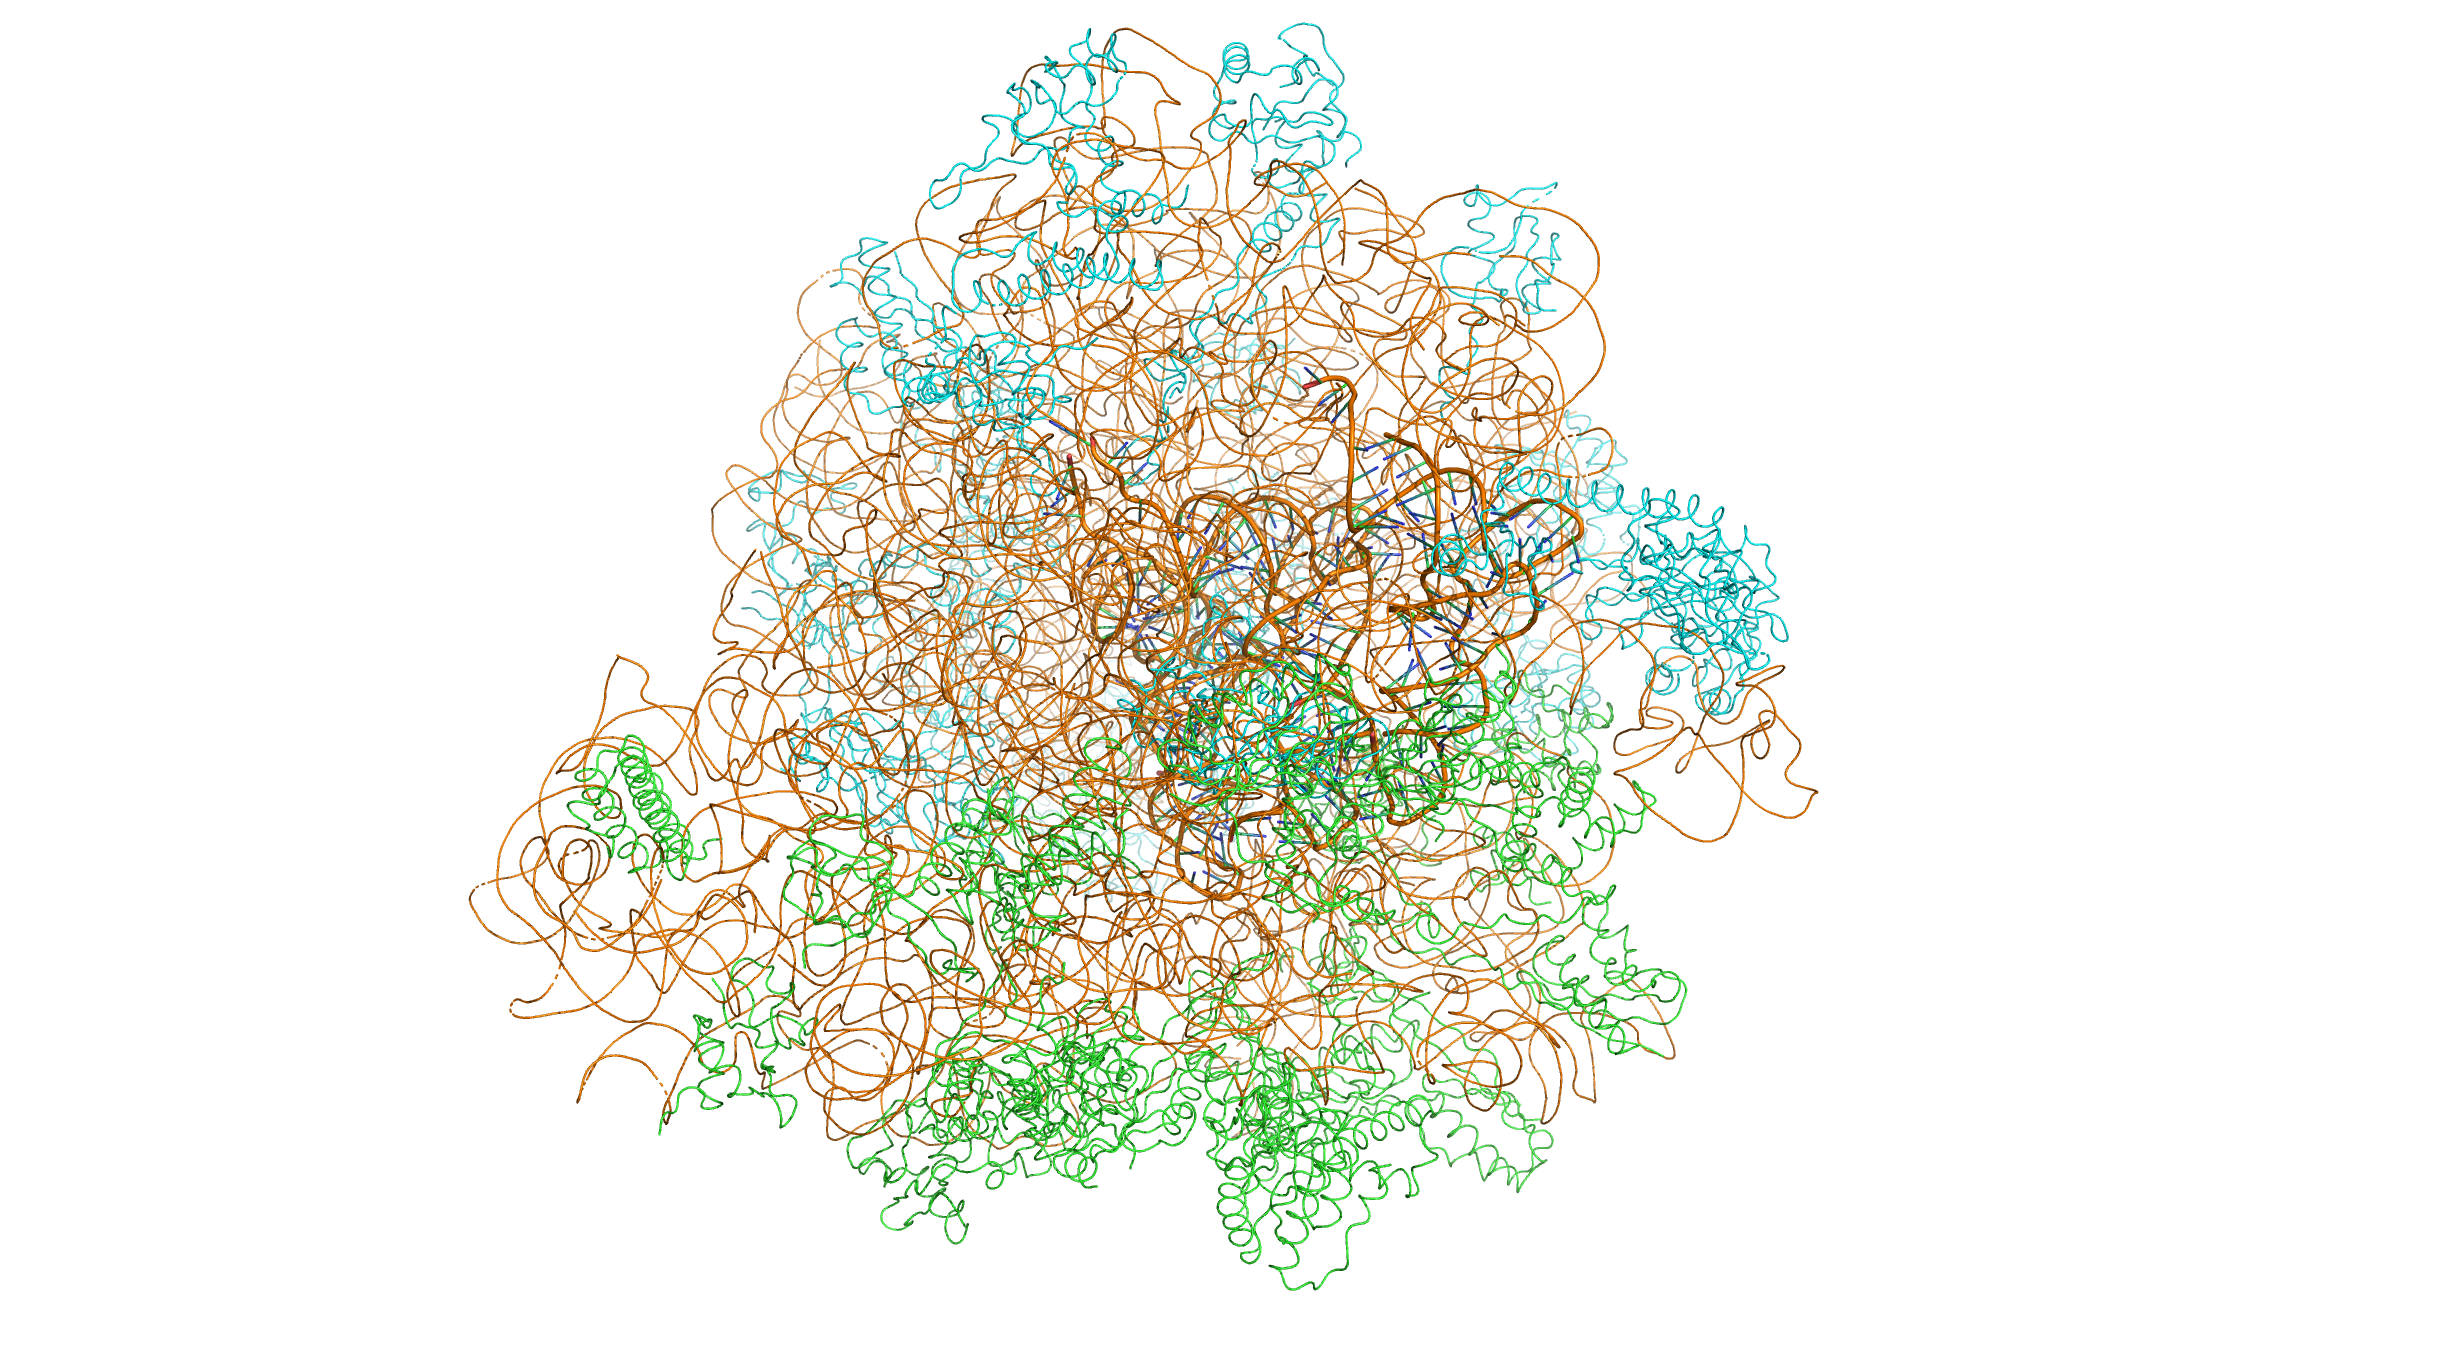
\includegraphics[width=0.7\linewidth]{./figures/translation/ttribosome} 

}

\caption{Crystal structure of the bacterial 70S ribosome of the bacterium \emph{Thermus thermophilus}. The 30S (small) ribosomal subunit proteins are colored in green, the 50S (large) subunit proteins are colored in blue, the ribosomal RNA is colored orange. The 30S subunits contains 3 tRNA molecules (based on atomic coordinates of \href{https://www.rcsb.org/structure/1jgq}{PDB 1JGQ} and \href{(https://www.rcsb.org/structure/1jgq)}{PDB 1GIY} rendered with open source molecular visualization tool PyMol.)}\label{fig:ttribosome}
\end{figure}

The unit of measurement used to describe the ribosomal subunits and the rRNA fragments is the Svedberg unit, a measure of the rate of sedimentation in centrifugation rather than size. This accounts for why fragment names do not add up: for example, bacterial 70S ribosomes are made of 50S and 30S subunits.

Bacteria have 70S ribosomes, each consisting of a small (30S) and a large (50S) subunit. \emph{Escherichia coli}, for example, has a 16S RNA subunit (consisting of 1540 nucleotides) that is bound to 21 proteins. The large subunit is composed of a 5S RNA subunit (120 nucleotides), a 23S RNA subunit (2900 nucleotides) and 31 proteins.

\hypertarget{eukaryotic-ribosomes}{%
\section{Eukaryotic ribosomes}\label{eukaryotic-ribosomes}}

Eukaryotes have 80S ribosomes located in their cytosol, each consisting of a small (40S) and large (60S) subunit. Their 40S subunit has an 18S RNA (1900 nucleotides) and 33 proteins. The large subunit is composed of a 5S RNA (120 nucleotides), 28S RNA (4700 nucleotides), a 5.8S RNA (160 nucleotides) subunits and 46 proteins.



\begin{figure}

{\centering 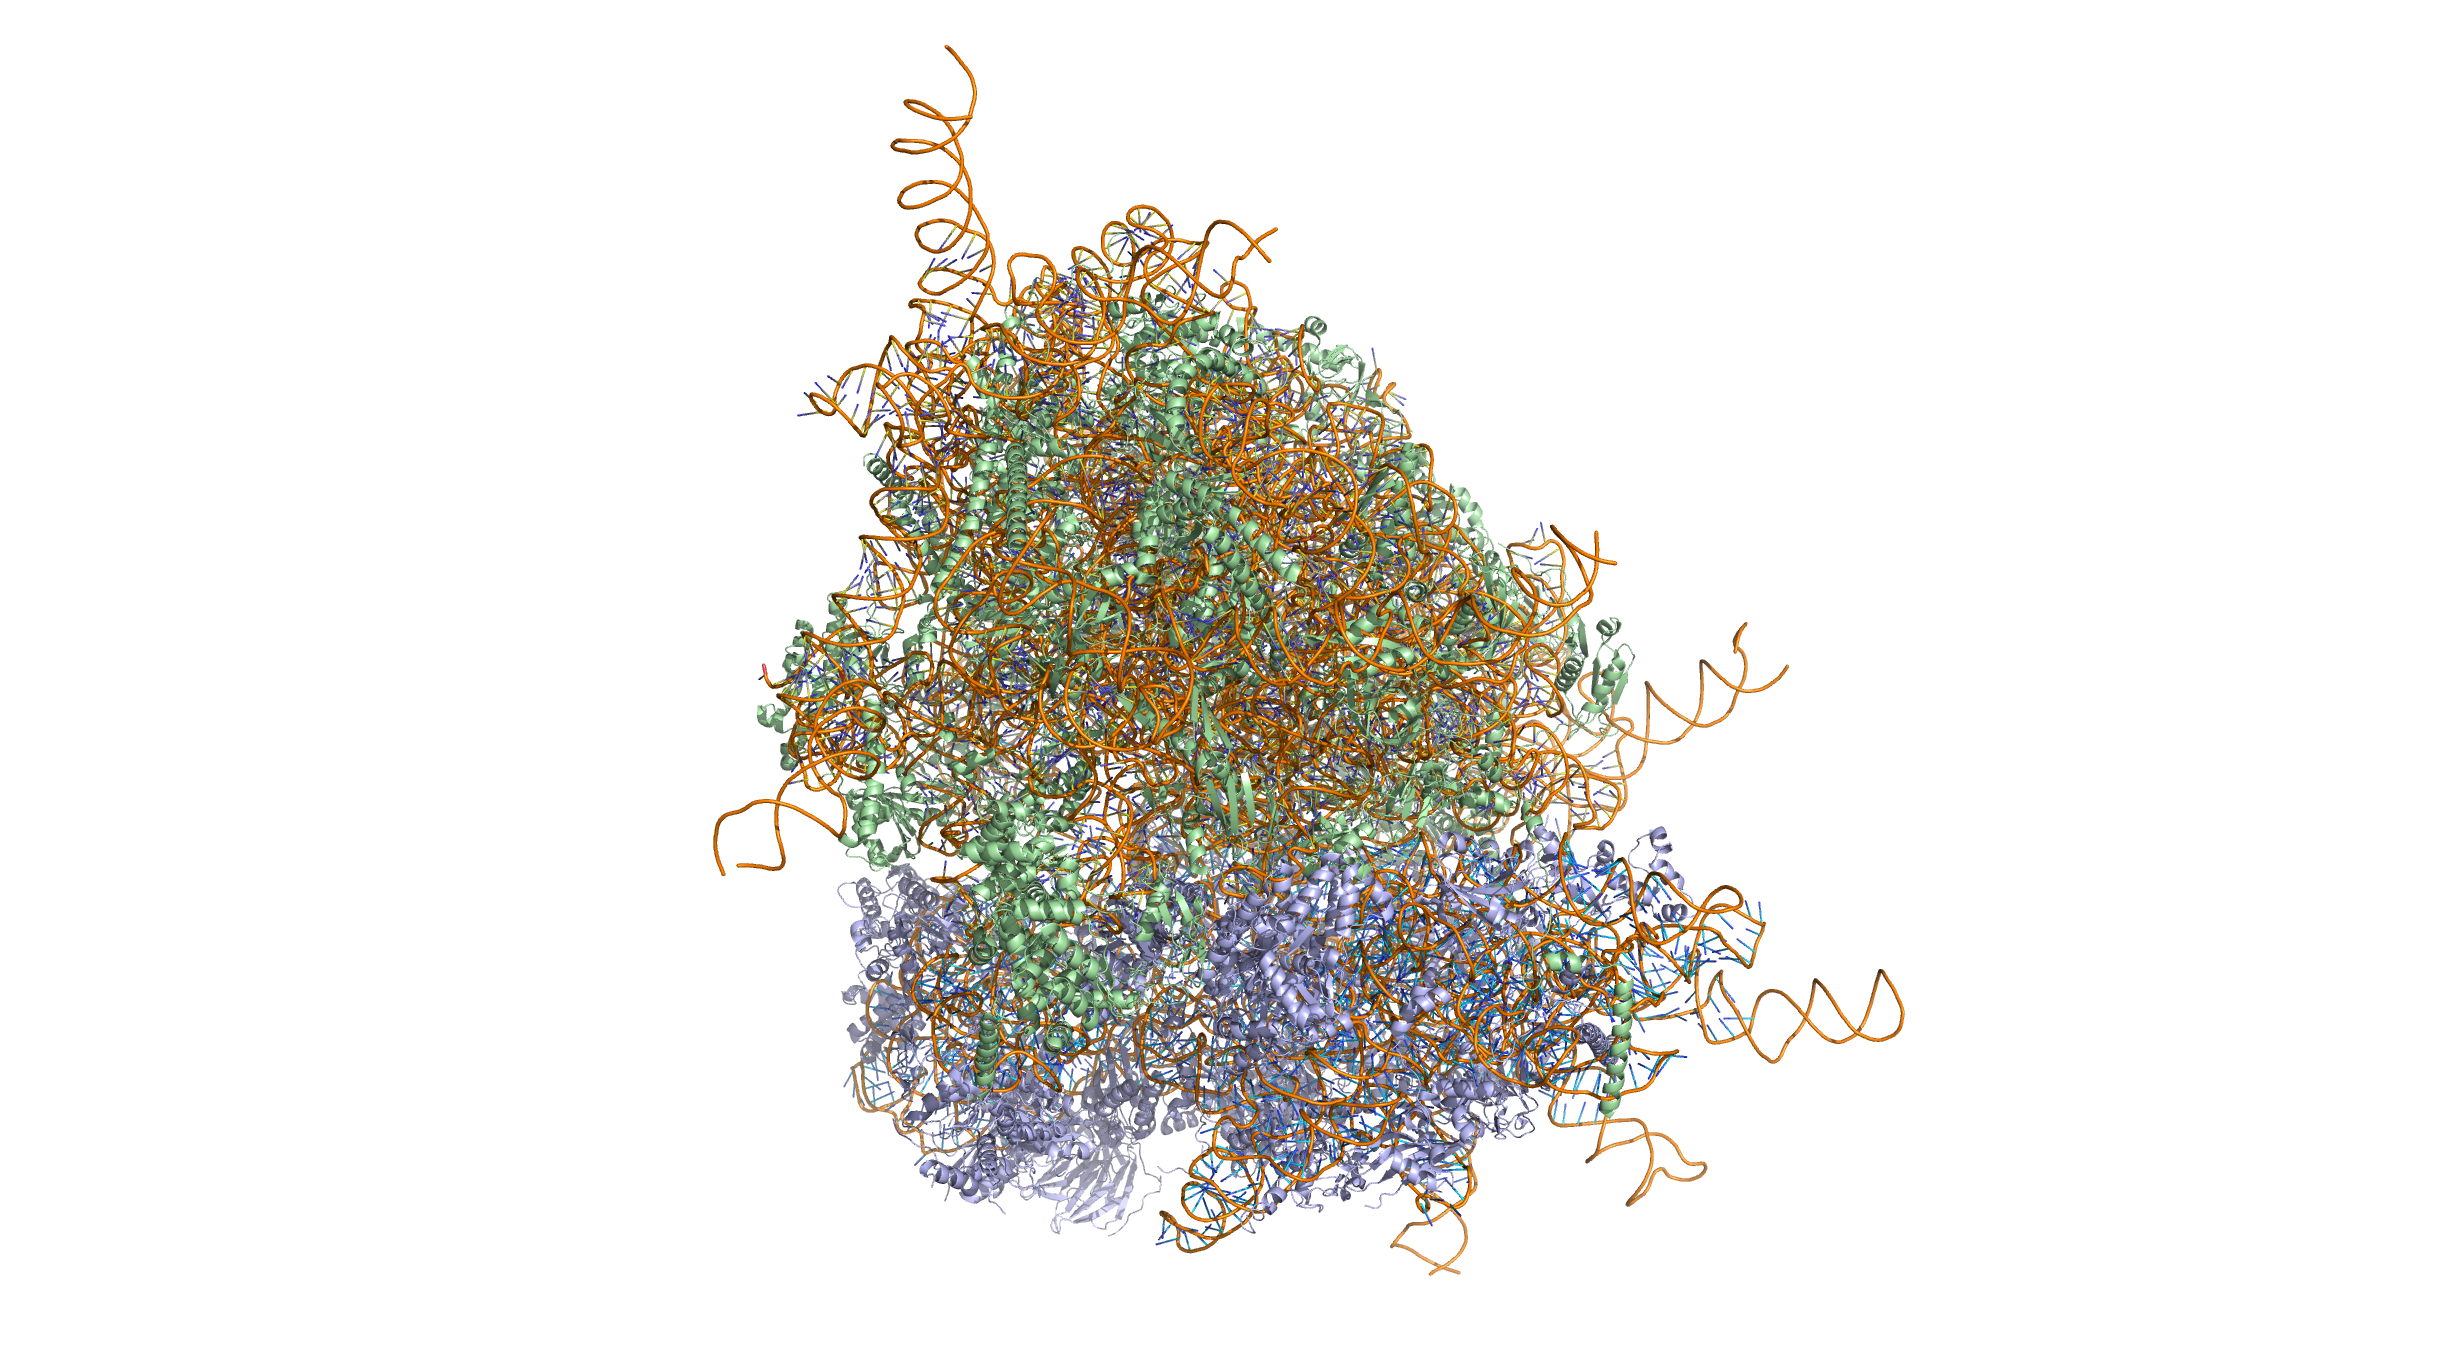
\includegraphics[width=0.7\linewidth]{./figures/translation/human_ribosome} 

}

\caption{Crystal structure of the human 80S ribosome (based on atomic coordinates of \href{https://www.rcsb.org/structure/4v6x}{PDB 4V6X} rendered with open source molecular visualization tool PyMol). The 40S (small) ribosomal subunit proteins are shown in lightblue, the 60S (large) subunit proteins in palegreen, the ribosomal RNA in orange.}\label{fig:ribosome}
\end{figure}

The differences between the bacterial and eukaryotic ribosomes are exploited by pharmaceutical chemists to create antibiotics that can destroy a bacterial infection without harming the cells of the infected person. Due to the differences in their structures, the bacterial 70S ribosomes are vulnerable to these antibiotics while the eukaryotic 80S ribosomes are not. Even though mitochondria possess ribosomes similar to the bacterial ones, mitochondria are not affected by these antibiotics because they are surrounded by a double membrane that does not easily admit these antibiotics into the organelle. The same cannot be said of chloroplasts, where antibiotic resistance in ribosomal proteins is a trait to be introduced as a marker in genetic engineering.

The various ribosomes share a core structure, which is quite similar despite the large differences in size. Much of the RNA is highly organized into various tertiary structural motifs, for example pseudoknots that exhibit coaxial stacking. The extra RNA in the larger ribosomes is in several long continuous insertions, such that they form loops out of the core structure without disrupting or changing it. All of the catalytic activity of the ribosome is carried out by the RNA; the proteins reside on the surface and seem to stabilize the structure.

A ribosome is made up of a subunit, a small 40S subunit or a large 60S subunit. These subunits come together before translation of mRNA into a protein to provide a location for translation to be carried out and a polypeptide to be produced. The choice of amino acid type to be added is determined by the genetic code on the mRNA molecule. Each amino acid added is matched to a three nucleotide subsequence of the mRNA. For each such triplet possible, the corresponding amino acid is accepted. The successive amino acids added to the chain are matched to successive nucleotide triplets in the mRNA. In this way, the sequence of nucleotides in the template mRNA chain determines the sequence of amino acids in the generated polypeptide. Addition of an amino acid occurs at the N-terminus of the peptide and thus translation is said to be amino-to-carboxyl directed.

The ribosome translates this code to a specific sequence of amino acids. The ribosome is a multi-subunit structure containing rRNA and proteins. It is the ``factory'' where amino acids are assembled into proteins. tRNAs are small noncoding RNA chains (75-90 nucleotides) that transport amino acids to the ribosome. tRNAs have a site for amino acid attachment, and a site called an anticodon. The anticodon is an RNA triplet complementary to the mRNA triplet that codes for their cargo amino acid.



\begin{figure}

{\centering 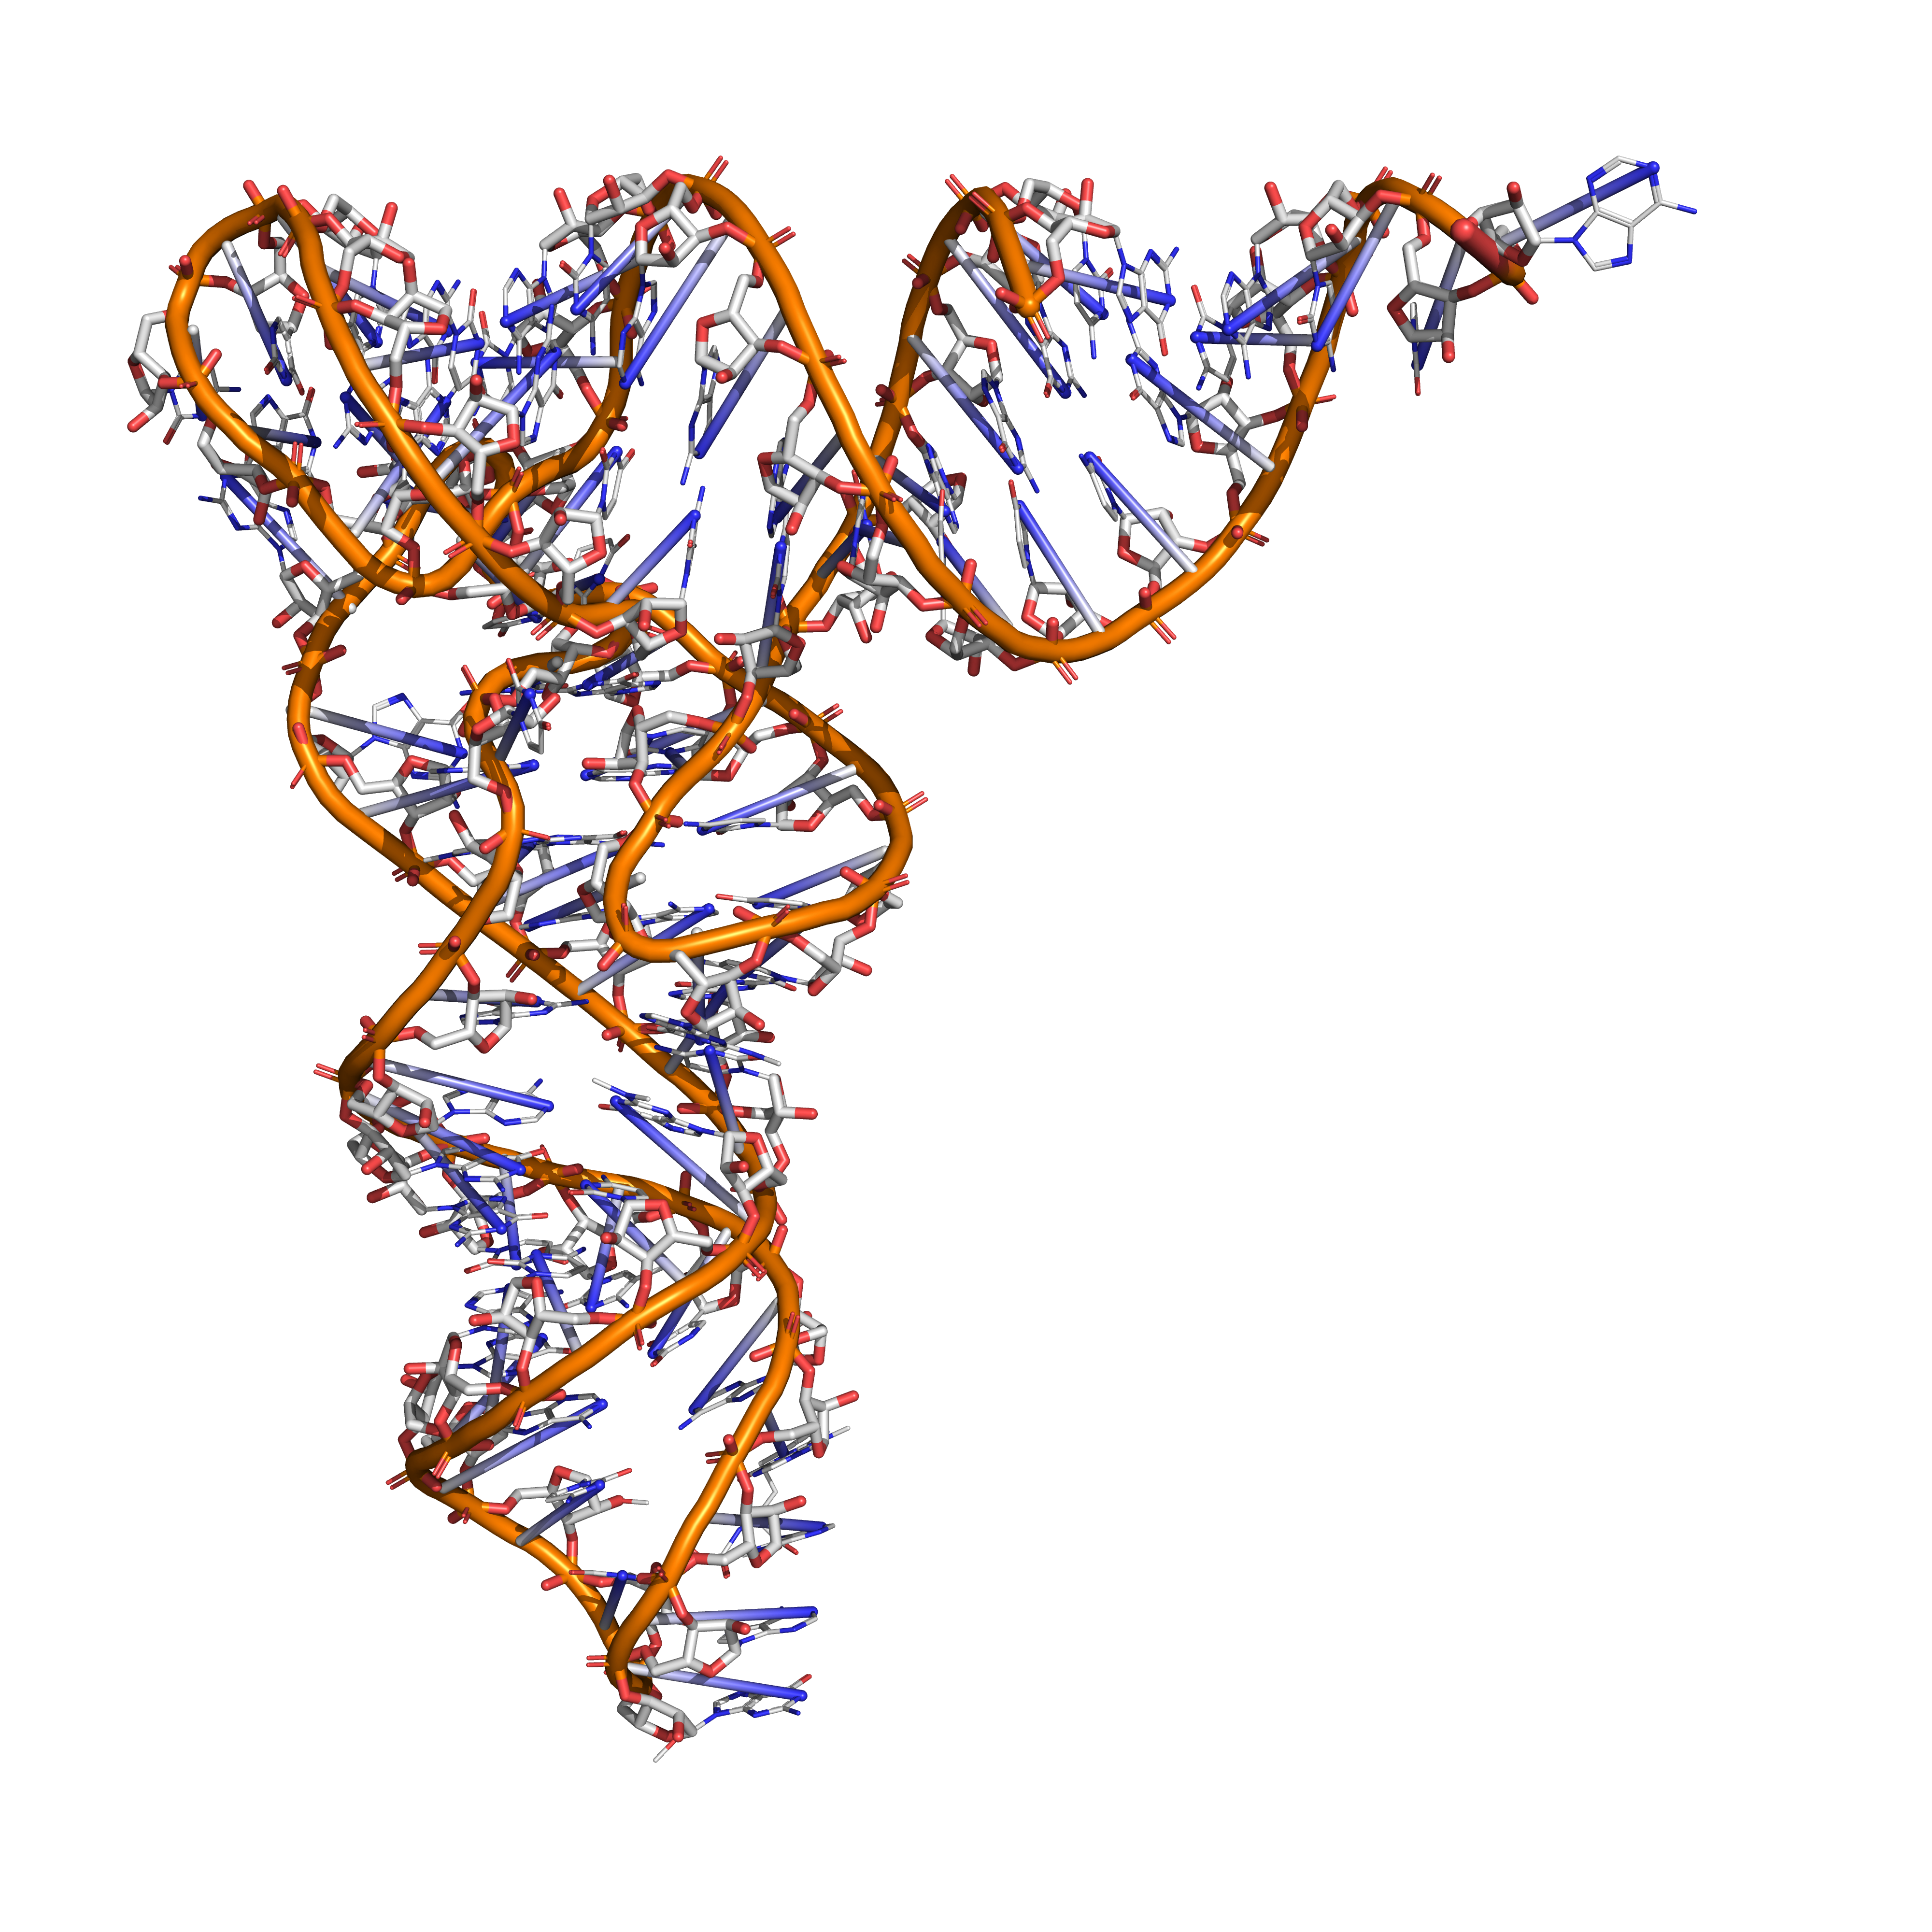
\includegraphics[width=0.7\linewidth]{./figures/translation/trna} 

}

\caption{Tertiary structure of tRNA (based on atomic coordinates of \href{https://www.rcsb.org/structure/1ehz}{PDB 1ehz} rendered with open source molecular visualization tool PyMol.)}\label{fig:trnastruc}
\end{figure}

Aminoacyl tRNA synthetases (enzymes) catalyze the bonding between specific tRNAs and the amino acids that their anticodon sequences call for. The product of this reaction is an aminoacyl-tRNA. In prokaryotes, this aminoacyl-tRNA is carried to the ribosome by EF-Tu, where mRNA codons are matched through complementary base pairing to specific tRNA anticodons. Aminoacyl-tRNA synthetases that mispair tRNAs with the wrong amino acids can produce mischarged aminoacyl-tRNAs, which can result in inappropriate amino acids at the respective position in protein. This ``mistranslation'' of the genetic code naturally occurs at low levels in most organisms, but certain cellular environments cause an increase in permissive mRNA decoding, sometimes to the benefit of the cell.

The ribosome has three sites for tRNA to bind. They are the aminoacyl site (abbreviated A), the peptidyl site (abbreviated P) and the exit site (abbreviated E). With respect to the mRNA, the three sites are oriented 5' to 3' E-P-A, because ribosomes move toward the 3' end of mRNA. The A-site binds the incoming tRNA with the complementary codon on the mRNA. The P-site holds the tRNA with the growing polypeptide chain. The E-site holds the tRNA without its amino acid, and the tRNA is then released. When an aminoacyl-tRNA initially binds to its corresponding codon on the mRNA, it is in the A site. Then, a peptide bond forms between the amino acid of the tRNA in the A site and the amino acid of the charged tRNA in the P site. The growing polypeptide chain is transferred to the tRNA in the A site. Translocation occurs, moving the tRNA in the P site, now without an amino acid, to the E site; the tRNA that was in the A site, now charged with the polypeptide chain, is moved to the P site. The tRNA in the E site leaves and another aminoacyl-tRNA enters the A site to repeat the process.

After the new amino acid is added to the chain, and after the mRNA is released out of the nucleus and into the ribosome's core, the energy provided by the hydrolysis of an ATP bound to the translocase EF-G (in prokaryotes) and eEF-2 (in eukaryotes) moves the ribosome down one codon towards the 3' end. The energy required for translation of proteins is significant. For a protein containing n amino acids, the number of high-energy phosphate bonds required to translate it is 4n+1. The rate of translation varies; it is significantly higher in prokaryotic cells (up to 17-21 amino acid residues per second) than in eukaryotic cells (up to 6-9 amino acid residues per second).

Even though the ribosomes are usually considered accurate, processive machines, the translation process is subject to errors that can lead either to the synthesis of erroneous proteins or to the premature abandonment of translation. The rate of error in synthesizing proteins has been estimated to be between 1/105 and 1/103 misincorporated amino acids, depending on the experimental conditions. The rate of premature translation abandonment, instead, has been estimated to be of the order of magnitude of 10−4 events per translated codon. The correct amino acid is covalently bonded to the correct transfer RNA (tRNA) by amino acyl transferases. The amino acid is joined by its carboxyl group to the 3' OH of the tRNA by an ester bond. When the tRNA has an amino acid linked to it, the tRNA is termed ``charged''. Initiation involves the small subunit of the ribosome binding to the 5' end of mRNA with the help of initiation factors (IF). In prokaryotes, initiation of protein synthesis involves the recognition of a purine-rich initiation sequence on the mRNA called the Shine-Dalgarno sequence. The Shine-Dalgarno sequence binds to a complementary pyrimidine-rich sequence on the 3' end of the 16S rRNA part of the 30S ribosomal subunit. The binding of these complementary sequences ensures that the 30S ribosomal subunit is bound to the mRNA and is aligned such that the initiation codon is placed in the 30S portion of the P-site. Once the mRNA and 30S subunit are properly bound, an initiation factor brings the initiator tRNA-amino acid complex, f-Met-tRNA, to the 30S P site. The initiation phase is completed once a 50S subunit joins the 30 subunit, forming an active 70S ribosome. Termination of the polypeptide occurs when the A site of the ribosome is occupied by a stop codon (UAA, UAG, or UGA) on the mRNA. mRNA usually cannot recognize or bind to stop codons. Instead, the stop codon induces the binding of a release factor protein (RF1 \& RF2) that prompts the disassembly of the entire ribosome/mRNA complex by the hydrolysis of the polypeptide chain from the peptidyl transferase center of the ribosome. Drugs or special sequence motifs on the mRNA can change the ribosomal structure so that near-cognate tRNAs are bound to the stop codon instead of the release factors. In such cases of `translational readthrough', translation continues until the ribosome encounters the next stop codon.

The process of translation is highly regulated in prokaryotic and eukaryotic organisms. Regulation of translation can impact the global rate of protein synthesis which is closely coupled to the metabolic and proliferative state of a cell. In addition, recent work has revealed that genetic differences and their subsequent expression as mRNAs can also impact translation rate in an RNA-specific manner.

\hypertarget{genetic-code-1}{%
\section{Genetic code}\label{genetic-code-1}}

Whereas other aspects such as the 3D structure, called tertiary structure, of protein can only be predicted using sophisticated algorithms, the amino acid sequence, called primary structure, can be determined solely from the nucleic acid sequence with the aid of a translation table.

\begingroup\fontsize{7}{9}\selectfont

\begin{longtable}[t]{>{\bfseries}ccccc>{\bfseries}c}
\caption{\label{tab:geneticcode}The genetic code: RNA codons.}\\
\toprule
 & U & C & A & G & \\
\midrule
\rowcolor{gray!6}   & UUU Phenylalanine (Phe) & UCU Serine (Ser) & UAU Tyrosine (Tyr) & UGU Cysteine (Cys) & U\\

 & UUC Phe & UCC Ser & UAC Tyr & UGC Cys & C\\

\rowcolor{gray!6}   & UUA Leucine (Leu) & UCA Ser & UAA STOP & UGA STOP & A\\

\multirow{-4}{*}{\centering\arraybackslash U} & UUG Leu & UCG Ser & UAG STOP & UGG Tryptophan (Trp) & G\\
\cmidrule{1-6}
\rowcolor{gray!6}   & CUU Leucine (Leu) & CCU Proline (Pro) & CAU Histidine (His) & CGU Arginine (Arg) & U\\

 & CUC Leu & CCC Pro & CAC His & CGC Arg & C\\

\rowcolor{gray!6}   & CUA Leu & CCA Pro & CAA Glutamine (Gln) & CGA Arg & A\\

\multirow{-4}{*}{\centering\arraybackslash C} & CUG Leu & CCG Pro & CAG Gln & CGG Arg & G\\
\cmidrule{1-6}
\rowcolor{gray!6}   & AUU Isoleucine (Ile) & ACU Threonine (Thr) & AAU Asparagine (Asn) & AGU Serine (Ser) & U\\

 & AUC Ile & ACC Thr & AAC Asn & AGC Ser & C\\

\rowcolor{gray!6}   & AUA Ile & ACA Thr & AAA Lysine (Lys) & AGA Arginine (Arg) & A\\

\multirow{-4}{*}{\centering\arraybackslash A} & AUG Methionine (Met) or START & ACG Thr & AAG Lys & AGG Arg & G\\
\cmidrule{1-6}
\rowcolor{gray!6}   & GUU Valine Val & GCU Alanine (Ala) & GAU Aspartic acid (Asp) & GGU Glycine (Gly) & U\\

 & GUC (Val) & GCC Ala & GAC Asp & GGC Gly & C\\

\rowcolor{gray!6}   & GUA Val & GCA Ala & GAA Glutamic acid (Glu) & GGA Gly & A\\

\multirow{-4}{*}{\centering\arraybackslash G} & GUG Val & GCG Ala & GAG Glu & GGG Gly & G\\
\bottomrule
\end{longtable}
\endgroup{}

There are many computer programs capable of translating a DNA/RNA sequence into a protein sequence. Normally this is performed using the Standard Genetic Code (Table \ref{tab:geneticcode}), however, few programs can handle all the ``special'' cases, such as the use of the alternative initiation codons. For instance, the rare alternative start codon CTG codes for Methionine when used as a start codon, and for Leucine in all other positions.


